\documentclass[a4paper, 12pt]{article}

\usepackage[top=2cm, bottom=2cm, left=2.5cm, right=2.5cm]{geometry}
\usepackage[utf8]{inputenc}
\usepackage{array}
\usepackage{verbatim}
\usepackage{graphicx}
\usepackage{hyperref}

\graphicspath{{img/}}

\begin{document}
\begin{flushleft}
\includegraphics{logo}\\
\textbf{UNIVERSIDADE ESTADUAL DE PONTA GROSSA} \\
SISTEMA UNIVERSIDADE ABERTA DO BRASIL - UAB \\
\underline{Licenciatura em Matemática | Polo UAB em Jacarezinho}\end{flushleft} \\
\textbf{ALUNO:} Ricardo Medeiros da Costa Junior   \textbf{RA:} 151774301 \\
\textbf{DISCIPLINA:} Instrumentação para o Ensino da Matemática III \\
\textbf{ATIVIDADE:} Tarefa atividade 2\end{flushleft} \\
\begin{enumerate}
\item Para compreender o conceito de aprendizagem significativa assista os vídeos:
  \begin{itemize}
  \item Professor Madruga - Aprendizagem Significativa
  \item Aprendizagem Significativa: do que estamos falando?
  \item Aprendizagem Significativa - a negociação dos sentidos
  \item A estrutura de uma aula significativa    
  \end{itemize}

  Em seguida responda as seguintes questões: 
  \begin{enumerate}
  \item O que diferencia aprendizagem significativa de outros tipos de aprendizagens? \\
    Segundo Ausubel a aprendizagem é significativa quando ela se relaciona com algo que aprendemos anteriormente. Em contrapartida, aprendizagem mecânica é a aprendizagem que nosso cérebro não consegue relacionar com nenhum conhecimento e por sua vez, tende a ser esquecida com maior facilidade.
    
  \item Como podemos definir sentido e significado? \\
    O sentido é subjetivo, está relacionado com as experiências e conhecimento de cada indivíduo, é definido por cada pessoa. O significado é uma construção social. É comum para todas as pessoas, é cientificamente embasado.
  \item Como transformar sentido em significado? \\
    Primeiramente, o diálogo para saber qual o sentido o aluno deu para determinado conteúdo, para posteriormente adequá-lo ao significado científico. O professor tem o papel de assessorar o aluno nessa trajetória. Para finalizar, quando o professor estiver montando seu plano de aula, o mesmo deve ficar atento em possíveis conteúdos que os alunos terão dificuldades e assim preparar atividades práticas para facilitar o processo de aprendizagem significativa por parte do aluno.
  \item O que é uma aula significativa e quais são as suas partes? \\
    Aula Significativa é uma aula estruturada de forma a facilitar o aluno a construir significado sobre o que ele está aprendendo. 1 - Construção de sentido; 2 - Apresentação do conteúdo; 3 - Verificação da aprendizagem.
  \item Como o professor pode ajudar o aluno a construir sentido e significado? \\
    Na construção de sentido, devemos contextualizar o conceito o mais próximo possível da realidade do aluno, o professor deve estar aberto ao diálogo, para saber qual o sentido que o aluno está formando sobre o conteúdo. A construção de significado é realizada na segunda parte da aula significativa. A construção deve ser feita a levar o aluno a construir o significado junto com o professor. O professor pode oferecer situações contextuais inclusivas para que o cérebro realize a assimilação do conceito.
  \end{enumerate}

\item Nas afirmativas abaixo complete os espaços em branco com as expressões: \\\\
  (AS) para \underline{Aprendizagem Significativa}\\
  (AM) para \underline{Aprendizagem Mecânica}\\\\
  (AS) A aprendizagem ocorre por descoberta.\\
  (AM) O novo conhecimento não considera os conhecimentos prévios do aluno\\
  (AM) O novo conhecimento não é integrado a conceitos existentes na estrutura significativa do aluno.\\
  (AM) Práticas, exercícios e réplicas reflexivas não contribuem para aprendizagem.\\
  (AM) A aprendizagem ocorre somente por recepção.
\item Faça um estudo cuidadoso do Texto ``A Teoria da Aprendizagem Significativa'' e responda as questões abaixo.
  \begin{enumerate}
  \item O que fundamenta a Teoria da Aprendizagem Significativa? Qual é sua premissa? Explique em até 10 linhas.\\
    Baseia-se na premissa que a mente humana possui uma estrutura organizada e hierarquizada de conhecimentos e ideias. Essa teoria caracteriza-se pela interação de uma informação com um aspecto relevante da estrutura cognitiva do sujeito. Uma informação é aprendida de forma significativa quando se relaciona com outras ideias que estejam disponíveis na mente do sujeito de modo que funcionem como âncoras.
  \item Como Ausubel conceitua aprendizagem mecânica e significativa? Elas se contrapõem? Explique em até 10 linhas.\\
    Segundo Ausubel a aprendizagem é significativa quando ela se relaciona com algo que aprendemos anteriormente. No entanto, aprendizagem mecânica é a aprendizagem que nosso cérebro não consegue relacionar com nenhum conhecimento e por sua vez, tende a ser esquecida com maior facilidade. Ausubel não vê oposição entre a aprendizagem mecânica e a significativa, mas as vê com um processo contínuo. Em alguns casos a aprendizagem mecânica é inevitável, mas posteriormente ela pode se transformar em significativa.
    
  \item O que são os subsunçores (subordinados ou integradores) segundo Ausubel?\\
    São ideias que proporcionam ancoragem, deias de base que os alunos possuem mas não estão ativadas. 
  \item Diferencie aprendizagem por recepção e por descoberta. Explique detalhadamente.\\
    Na aprendizagem receptiva, a informação é apresentada ao aluno em sua forma final, já na aprendizagem por descoberta, o conteúdo a ser aprendido necessita ser descoberto pelo aluno. A aprendizagem por descoberta pressupõe que o próprio indivíduo descubra o conhecimento dependendo de seus próprios recursos. Ausubel salienta que o custo-benefício para aprendizagens por descoberta é pouco considerável, excepto por alguns casos em uma tarefa de aprendizagem difícil, que o aprendiz carece de uma sofisticação mínima num campo determinado de conhecimento. Os dois tipos de aprendizagens podem ser significativas, no entando seria inviável utilizar aprendizagem por descoberta regularmente pois seria necessário disponibilidade de tempo.\\
    Ausubel não vê uma relação direta em aprendizagem mecânica e a aprendizagem por recepção. Para ele, a aprendizagem receptiva-significativa é um processo ativo, mas deve antender alguns requisitos para ser efetuado; como uma análise de conhecimentos prévio do aluno, por exemplo.\\
    Para Ausubel, o máximo da aprendizagem significativa seria aquela que resulta da pesquisa científica, pois se situa no extremo dos dois contínuos, advém da combinação entre aprendizagem por descoberta autônoma e aprendizagem significativa.
  \end{enumerate}

\item Este com atenção os textos
  \begin{itemize}
  \item Mapas conceituais e aprendizagem significativa
  \item Uma abordagem para o ensino da lógica - mapas conceituais
    \\\\ e assista atentamente os vídeos:\\
  \item Mapas Conceituais no Ensino da Matemática
  \item Mapas Conceituais - Utilizando o Cmap Tools
  \item Mapa Conceitual no Word
  \item Introdução aos Mapas Conceituais Aplicados à Educação\\
  \end{itemize}
  
  \textbf{Em seguida responda as questões:}
  \begin{enumerate}
  \item O que são mapas conceituais?\\\\
    São diagramas de significados, de relações significativas e de hierarquias conceituais. Não deve ser confundidos com organogramas, diagramas de fluxo porque não implicam uma sequência. Não podem ser confundidos com mapas mentais que são associacionistas, pois não se ocupam de relações entre conceitos, englobam coisas que não são conceitos e não estão organizados hierarquicamente. Também não podem ser confundidos com quadros sinópticos, pois não buscam classificas os conceitos, mas relacioná-los.
  \item Como os mapas conceituais podem constituir-se de ferramentas de ensino para o professor e aprendizagem para o aluno?\\\\
    Para os professores os mapas conceituais constituem-se em poderosos auxiliares nas suas tarefas rotineiras, como por exemplo tornar claro os conceitos difíceis para os alunos, organização dos conteúdos em uma ordem sistemática, auxilia para que mantenham mais atenção nos conceitos chaves e nas relações entre eles. Quando utilizados por um estudante faz com que ele comece a pensar no desenvolvimento via um mapa, ele se obriga a não só entender os assuntos, mas a fazer as relações entre esse determinado assunto a outros, levando dinamismo a aula.
  \item Nas Diretrizes Curriculares do Paraná para o ensino de Matemática, estão definidos os conteúdos estruturantes agrupados em cinco áreas de conhecimento: Números e Álgebra; Grandezas e Medidas; Geometrias; Funções e Tratamento da Informação. Considerando os conteúdos básicos definidos para a área de Números e Álgebra para o ensino fundamental – segundo segmento, 6º ao 9º ano, elabore um mapa conceitual que represente o estudo desses conteúdos matemáticos nos quatros anos, bem como suas inter-relações. \\\\
      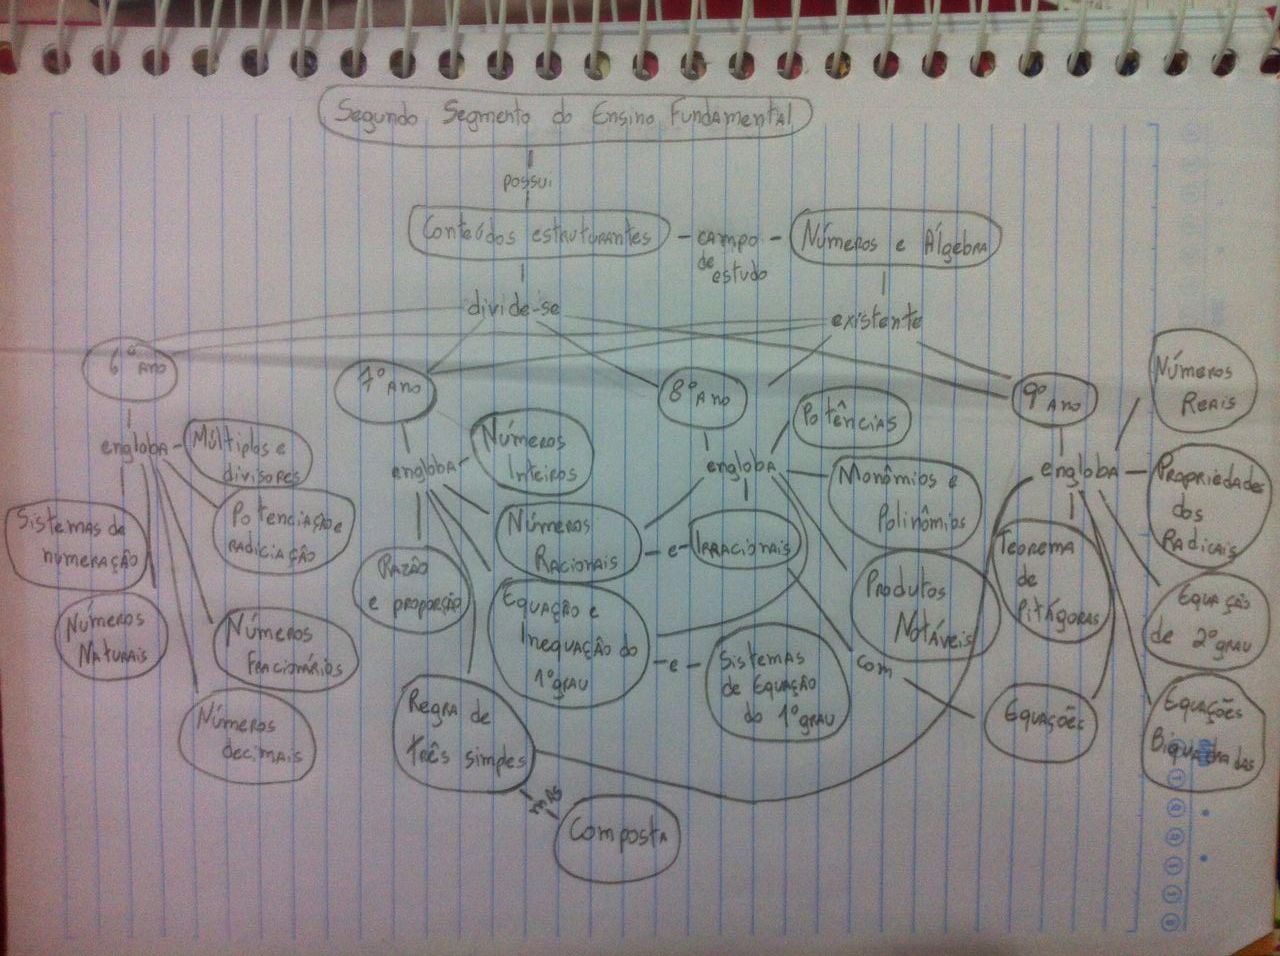
\includegraphics[width=1\textwidth]{1}

  \end{enumerate}   
\end{enumerate}
\end{document}
